\documentclass[12pt,a4paper]{exam}
\usepackage[utf8]{inputenc}
\usepackage[T1]{fontenc}
\usepackage{amsmath}
\usepackage{amsfonts}
%\usepackage{amssymb}
\usepackage{graphicx}
\usepackage{geometry}
\usepackage{enumitem}

\geometry{a4paper, margin=2cm}

\usepackage{cprotect}

\usepackage{xcolor}
\definecolor{maroon}{cmyk}{0, 0.87, 0.68, 0.32}
\definecolor{halfgray}{gray}{0.55}
\definecolor{ipython-frame}{RGB}{207, 207, 207}
\definecolor{ipython-bg}{RGB}{247, 247, 247}
\definecolor{ipython-red}{RGB}{186, 33, 33}
\definecolor{ipython-green}{RGB}{0, 128, 0}
\definecolor{ipython-cyan}{RGB}{64, 128, 128}
\definecolor{ipython-purple}{RGB}{170, 34, 255}
\usepackage{listings}
\lstdefinelanguage{iPython}{
	morekeywords={access,and,del,except,exec,in,is,lambda,not,or,raise},
	morekeywords=[2]{for,print,abs,all,any,basestring,bin,bool,bytearray,callable,chr,classmethod,cmp,compile,complex,delattr,dict,dir,divmod,enumerate,eval,execfile,file,filter,float,format,frozenset,getattr,globals,hasattr,hash,help,hex,id,input,int,isinstance,issubclass,iter,len,list,locals,long,map,max,memoryview,min,next,object,oct,open,ord,pow,property,range,reduce,reload,repr,reversed,round,set,setattr,slice,sorted,staticmethod,str,sum,super,tuple,type,unichr,unicode,vars,xrange,zip,apply,buffer,coerce,intern,elif,else,if,continue,break,while,class,def,return,try,except,import,finally,try,except,from,global,pass, True, False},
	sensitive=true,
	morecomment=[l]\#,%
	morestring=[b]',%
	morestring=[b]",%
	moredelim=**[is][\color{black}]{@@}{@@},
	%%
	%morestring=[s]{'''}{'''},% used for documentation text (mulitiline strings)
	%morestring=[s]{"""}{"""},% added by Philipp Matthias Hahn
	%%
	%morestring=[s]{r'}{'},% `raw' strings
	%morestring=[s]{r"}{"},%
	%morestring=[s]{r'''}{'''},%
	%morestring=[s]{r"""}{"""},%
	%morestring=[s]{u'}{'},% unicode strings
	%morestring=[s]{u"}{"},%
	%morestring=[s]{u'''}{'''},%
	%morestring=[s]{u"""}{"""}%
	%
	% {replace}{replacement}{lenght of replace}
	% *{-}{-}{1} will not replace in comments and so on
	%literate=
	%{\%}{{{\color{ipython-purple}+}}}1,
	%{á}{{\'a}}1 {é}{{\'e}}1 {í}{{\'i}}1 {ó}{{\'o}}1 {ú}{{\'u}}1,
	%{Á}{{\'A}}1 {É}{{\'E}}1 {Í}{{\'I}}1 {Ó}{{\'O}}1 {Ú}{{\'U}}1
	%{à}{{\`a}}1 {è}{{\`e}}1 {ì}{{\`i}}1 {ò}{{\`o}}1 {ù}{{\`u}}1
	%{À}{{\`A}}1 {È}{{\'E}}1 {Ì}{{\`I}}1 {Ò}{{\`O}}1 {Ù}{{\`U}}1
	%{ä}{{\"a}}1 {ë}{{\"e}}1 {ï}{{\"i}}1 {ö}{{\"o}}1 {ü}{{\"u}}1
	%{Ä}{{\"A}}1 {Ë}{{\"E}}1 {Ï}{{\"I}}1 {Ö}{{\"O}}1 {Ü}{{\"U}}1
	%{â}{{\^a}}1 {ê}{{\^e}}1 {î}{{\^i}}1 {ô}{{\^o}}1 {û}{{\^u}}1
	%{Â}{{\^A}}1 {Ê}{{\^E}}1 {Î}{{\^I}}1 {Ô}{{\^O}}1 {Û}{{\^U}}1
	%{œ}{{\oe}}1 {Œ}{{\OE}}1 {æ}{{\ae}}1 {Æ}{{\AE}}1 {ß}{{\ss}}1
	%{ç}{{\c c}}1 {Ç}{{\c C}}1 {ø}{{\o}}1 {å}{{\r a}}1 {Å}{{\r A}}1
	%{€}{{\EUR}}1 {£}{{\pounds}}1
	%
	%{^}{{{\color{ipython_purple}\^{}}}}1
	%{=}{{{\color{ipython_purple}=}}}1
	%%
	%*{-}{{{\color{ipython_purple}-}}}1
	%{*}{{{\color{ipython_purple}$^\ast$}}}1
	%{/}{{{\color{ipython_purple}/}}}1%%
	%{+=}{{{+=}}}1
	%{-=}{{{-=}}}1
	%{*=}{{{$^\ast$=}}}1
	%{/=}{{{/=}}}1,
	%
	identifierstyle=\color{black}\footnotesize\ttfamily,
	commentstyle=\color{ipython-cyan}\footnotesize\itshape\ttfamily,
	stringstyle=\color{ipython-red}\footnotesize\ttfamily,
	keepspaces=true,
	showspaces=false,
	showstringspaces=false,
	rulecolor=\color{ipython-frame},
	frame=single,
	frameround={t}{t}{t}{t},
	%framexleftmargin=6mm,
	%numbers=left,
	%numberstyle=\color{ipython-cyan},
	backgroundcolor=\color{ipython-bg},
	%   extendedchars=true,
	basicstyle=\footnotesize\ttfamily,
	keywordstyle=[2]\color{ipython-green}\bfseries\footnotesize\ttfamily, 
	keywordstyle=\color{ipython-purple}\bfseries\footnotesize\ttfamily
}

\lstdefinelanguage{iOutput} {
	sensitive=true,
	identifierstyle=\color{black}\small\ttfamily,
	stringstyle=\color{ipython-red}\small\ttfamily,
	keepspaces=true,
	showspaces=false,
	showstringspaces=false,
	rulecolor=\color{ipython-frame},
	%frame=single,
	%frameround={t}{t}{t}{t},
	%backgroundcolor=\color{ipython-bg},
	basicstyle=\small\ttfamily,
}

\lstnewenvironment{ipython}[1][]{\lstset{language=iPython,mathescape=true,escapeinside={*@}{@*}}%
}{%
}

\lstnewenvironment{ioutput}[1][]{\lstset{language=iOutput,mathescape=true,escapeinside={*@}{@*}}%
}{%
}

\title{Financial Market Course 22/23\\ Exam}
\author{Prof. Simone Freschi, Prof. Matteo Sani}
\date{$16^{\mathrm{th}}$ February 2023}

\printanswers
%\noprintanswers
\begin{document}
\maketitle
%\addpoints{exam}
\begin{center}
\fbox{\fbox{\parbox{5.5in}{\centering
Answer the questions in the spaces provided. If you run out of room for an answer, continue on the page back.}}}
\end{center}

\begin{center}
\vspace{5mm}
\makebox[0.75\textwidth]{Student's name:\enspace\hrulefill}
\end{center}

\section*{Questions}
\vspace{.5cm}
\begin{questions}
\question Describe the equation for the expected return for a horizon of 1y of a 10y bond (with a coupon \textbf{C}, duration \textbf{D} and convexity \textbf{Conv}) given the expectation of interest rate movements equal to $\delta r$.
\begin{enumerate}[label=(\alph*),font=\itshape]
\item What will happen if the curve is inverted (short rates are higher than long rates) such as in the USA now, if rates remain unchanged from now to the horizon? 
\item what will happen if the curve is upward sloping but there is a parallel shift in 1y time?
\end{enumerate}
\fillwithlines{3cm}
\begin{solution}
%%%% SOLUTION EX 1
\end{solution}

\question Describe the equation for the return attribution model by Brinson, Hood and Beebower (BHB). 
\begin{enumerate}[label=(\alph*),font=\itshape]
\item Explain the difference between Allocation Effect and Security Selection Effect 
\item Imagine that your portfolio is overweight Energy (30\% vs 20\% Benchmark) and the Energy sector is up 15\%. Your energy stocks in the portfolio are up only 5\%. Determine the allocation effect and the selection effect and the overall portfolio result.
\end{enumerate}
\fillwithlines{3cm}
\begin{solution}
%%%% SOLUTION EX 2
\end{solution}

%\question[15] 	Describe the price in real terms and nominal terms of an Inflation Linked Bond.
%\begin{enumerate}
%\item What will happen to the price if nominal rates rise of 1\% and inflation rises of 2\%.
%\item If real rates are 1\% and nominal rates are 5\% (so brekeven inflation is equal to 4\%). What will happen to the Inflation Linked Bond if breakevens go down of 1\% and real rates remain the same? And what will happen to a Nominal Bond with the same maturity?
%
%\end{enumerate}
%\fillwithlines{3cm}
%
%\question[15] Describe the asset swap contract for a coupon bond with coupons equal to \textbf{C} and dirty Price equal to $P(t)$.	
%\begin{enumerate}
%\item What will happen to the price if the spread increase, all the rest being equal? What does it mean in term of credit quality expectation by the market for the bond's issuer?
%\item What is the difference between asset swap spread and \textbf{G-spread} or \textbf{I-spread} calculated in Bloomberg screen?
%\end{enumerate}
%\fillwithlines{3cm}

%\question[20] What is \texttt{numpy} array ?
%\fillwithlines{3cm}
%\begin{solution}
%\texttt{numpy} arrays are array structure more flexible then standard \texttt{python} lists. By using \texttt{numpy} arrays reading and writing items is faster and more efficient.
%\end{solution}

\question What is the output of the below program ?
\begin{ipython}
>>> names = ['Chris', 'Jack', 'John', 'Daman']
>>> print(names[-1][-1])
\end{ipython}
\makeemptybox{3.cm}
%\vspace{\stretch{1}}
\begin{solution}
%%%% SOLUTION EX 3
The output is: 
\begin{ioutput}
n
\end{ioutput}
\end{solution}

%\question[20]
%How to generate random numbers in Python ?
%\makeemptybox{3cm}
%
%\begin{solution}
%We can generate random numbers using different functions in Python. They are:
%
%\begin{ipython}
%>>> import random
%>>> random.random()      # This command returns a floating point
%                         # number, between 0 and 1.
%>>> random.uniform(X, Y) # It returns a floating point 
%                         # number between the values 
%                         # given as X and Y.
%>>> random.randint(X, Y) # This command returns a random
%                         # integer between the values 
%                         # given as X and Y.
%\end{ipython}
%
%Alternatively it can be used the \texttt{numpy} package:
%
%\begin{ipython}
%>>> import numpy as np
%>>> np.random.normal() # Normal distributed random number
%\end{ipython}
%\end{solution}

\question
How to print in \texttt{python} the sum of the numbers between 1 and 100 included ?
\makeemptybox{3cm}

\begin{solution}
%%%% SOLUTION EX 4
We can print sum of the numbers starting from 1 to 100 using this code:

\begin{ipython}
>>> print (sum(range(1, 101)))
\end{ipython}
\begin{ioutput}
5050
\end{ioutput}
\end{solution}

%\question[20]
%What is the following program output ?
%\begin{ipython}
%>>> names1 = ['Amir', 'Bear', 'Charlton', 'Daman']
%>>> names2 = names1
%>>> names3 = names1[:]
%
%>>> names2[0] = 'Alice'
%>>> names3[1] = 'Bob'
%
%>>> sum = 0
%>>> for ls in (names1, names2, names3):
%>>> 	if ls[0] == 'Alice':
%>>>    		sum += 1
%>>> 	if ls[1] == 'Bob':
%>>>    		sum += 10
%
%>>> print (sum)
%\end{ipython}
%\makeemptybox{3cm}
%
%\begin{solution}
%The output is:
%\begin{ioutput}
%12
%\end{ioutput}
%\end{solution}

\question Write a \texttt{python} program to find the second largest number in a list.
\makeemptybox{3cm}

\begin{solution}
%%%% SOLUTION EX 5
Python program to find the second largest number in a list:

\begin{ipython}
>>> a = [69, 98, 17, 0, 70, 24, 89, 62, 1, 6, 100, 75, 45, 59, 22]
>>> print ("Second largest element is:", sorted(a)[-2])
\end{ipython}
\end{solution}

%\question[20] A portfolio has a daily return variation distribution as shown in the following figure. The picture also indicates the \textbf{5\% area} under the distribution. 
%Based on the graph estimate the \textbf{2 days 95\%-VaR} and the \textbf{1 day 95\%-Expected Shortfall} values. 
%Briefly justify the approximate numbers.
%\begin{center}
%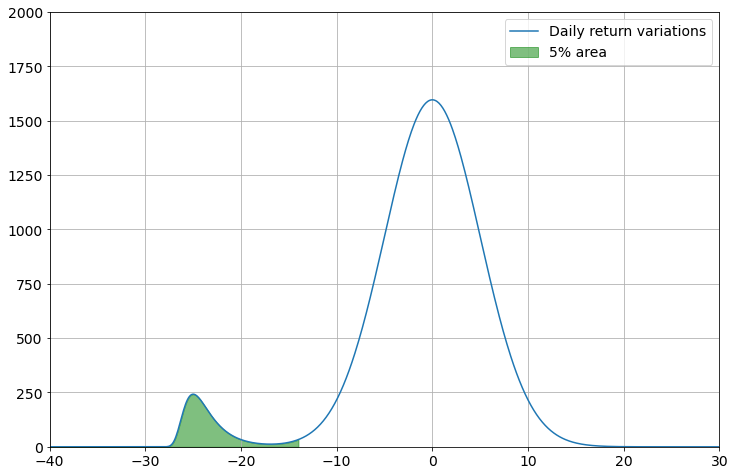
\includegraphics[width=0.8\textwidth]{var}
%\end{center}
%\makeemptybox{3cm}
%
%\begin{solution}
%2 days 95\%-VaR = $14 * \sqrt{2} \approx 19.8$, 1 day 95\%-ES $\approx 23$
%\end{solution}

\question Consider an interest rate swaption whose value is about 1450000 EUR. The price has been determined with Monte Carlo involving the simulation of 100 scenarios and is quoted with an error of 1.5\%. Unfortunately this is not enough for your purposes since you need to reach a precision of 0.1\%.

How many Monte Carlo experiments you need to run to achieve your goal ?

\makeemptybox{1.5 cm}

\begin{solution}
%%%% SOLUTION EX 6
$N_{new} = \left(\cfrac{0.015}{0.001}\right)^{2}*100 = 22500$
\end{solution}

\question Imagine to have two sets of CDS of various maturities on the same reference entity (Risky Corp.) but differing in currency: one set in EUR, the other in USD.

Bootstrapping the two sets you can derive two \textbf{credit curves} referring to Risky Corp., how different will be the two curves ? (Comment your answer.)

\fillwithlines{3cm}

\begin{solution}
%%%% SOLUTION EX 7
Observed differences in the credit curves are mostly driven by the correlation between the default risk of the obligor and the exchange rate.
\end{solution}
%\newpage
%\begin{center}
%\gradetable[h][questions]
%\end{center}
\end{questions}
\end{document}
